%% Floats of the Introduction (Fig. 1).  The prose is in 01_intro.tex.

\begin{figure}
\centering
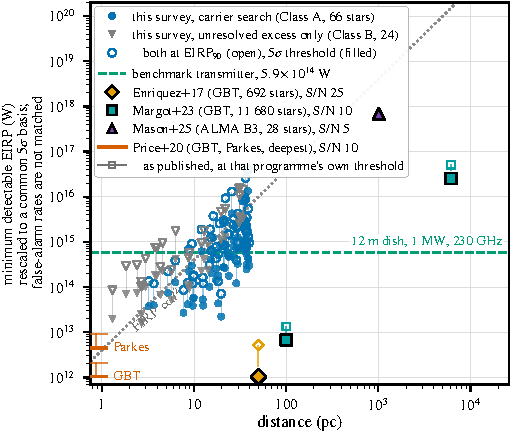
\includegraphics[width=\columnwidth]{figures/eirp_context_a.pdf}\\
{\footnotesize (a)}\\[4pt]
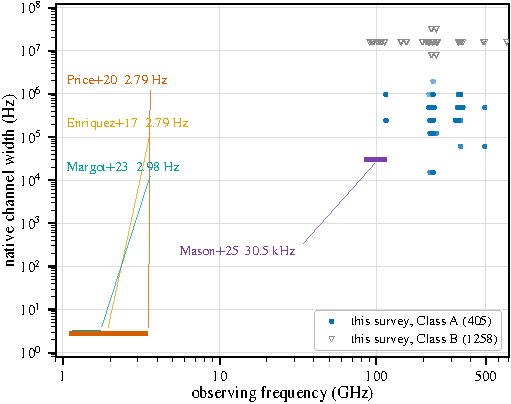
\includegraphics[width=\columnwidth]{figures/eirp_context_b.pdf}\\
{\footnotesize (b)}
\caption{Where this survey sits among published radio technosignature
searches (\S\ref{sec:intro}). \textbf{(a)} Minimum detectable EIRP against distance;
this survey's deepest window per star -- blue, the carrier search; grey,
coarse channels only; filled, the bare threshold; open,
$\mathrm{EIRP}_{90}$. \textbf{(b)} Native channel width against sky
frequency (filled, Class~A; open, Class~B).}
\label{fig:context}
\end{figure}
